\chapter{Analiza Teoretyczna problemu}
\label{chapter-2}
\section{Model systemu}

Z uwagi na to, że litera "x" jest wielokrotnie używana w opisie modelu autor pracy zdecydował się na wstępie wprowadzić krótką legendę używanych oznaczeń z tą literą:
\begin{itemize}
    \item $x$ pisane czcionką typu $italic$ oznacza współrzędną w układzie kartezjańskim
    \item $\mathrm{x(t)}$ lub $\mathrm{x(n)}$ oznaczają sygnał w dziedzinie czasu (ciągłej lub dyskretnej)
    \item $\mathrm{X}(f)$, $\mathrm{X(k)}$ oznacza reprezentację tego samego sygnału w dziedzinie częstotliwości, zaś $\mathrm{X(k,n)}$ w dziedzinie krótkoczasowej transformaty Fouriera.
    \item $\bm{\mathrm{x}}(f)$, $\bm{\mathrm{x}}(k)$ lub $\bm{\mathrm{x}}(k,n)$ pisane pogrubioną czcionką oznacza wektor o długości $M$ reprezentujący sygnał na $M$ mikrofonach odpowiednio dziedzinach częstotliwości i krótkoczasowej transformaty Fouriera.
\end{itemize}


\noindent Na wstępie postanawia się intujcyjnie przedstawić pochodzenie wzorów użytych poniżej. W szczególności interesujący jest wektor sterujący $\bm{\mathrm{a}}$.

\noindent Zakłada się, że źródła znajdują się w sferze dalekiej, tj. odległość źródła od mikrofonu jest znacznie większa od długości fali i fizycznych wymiarów mikrofonu. Co więcej zakłada się, że mikrofony są na tyle blisko siebie, że nie występuje pomiędzy nimi tłumienie.

\noindent Na mikrofon pada sygał nadchodzący z kierunku $\theta_{l}$.
Zapis sygnału w punkcie $\bm{\mathrm{d}}_{0} = [0,0]$ to $\mathrm{x}_{l}(t,\bm{\mathrm{d}}_{0})$. Opóźnienie w czasie tego sygnału na mikrofonie położonym w $\bm{\mathrm{d}}_{\mathrm{m}} = [x_{\mathrm{m}},y_{\mathrm{m}}]$ względem punktu $\bm{\mathrm{d}}_{0}$ wynosić będzie zatem pewne $\tau$. Różnica dróg między punktami wyniesie $\Delta d$ tak jak na rysunku \ref{fig:direction}. Za pomocą prostej trygonometrii może zostać udodnione, że:
\begin{equation}
    \label{equation:2.4}
    \Delta d = -x_{\mathrm{m}}\cos{\theta_{l}} - y_{\mathrm{m}}\sin{\theta_{l}}
\end{equation}
Następnie przyjmując prędkość rozchodzenia się fali w ośrodku $c$ można zapisać, że:
\begin{equation}
    \label{equation:2.5}
    \tau = \dfrac{\Delta d}{c}
\end{equation}

\noindent Przechodząc z sygnałem do dziedziny częstotliwości i zakładając parę transformat Fouriera $\mathrm{x}_{l}(t,\bm{\mathrm{d}}_{0})\xleftrightarrow{}\mathrm{X}_{l}(f,\bm{\mathrm{d}}_{0})$ można zapisać, że:
\begin{equation}
    \label{equation:2.6}
    \mathrm{x}_{l}(t,\bm{\mathrm{d}}_{\mathrm{m}}) \xleftrightarrow{} \mathrm{X}_{l}(f,\bm{\mathrm{d}}_{0})e^{j 2 \pi f \tau} =
    \mathrm{a}_{l}(f,\bm{\mathrm{d}}_{\mathrm{m}}) \mathrm{X}_{l}(f,\bm{\mathrm{d}}_{0}) 
\end{equation}

\noindent W przypadku wielu mikrofonów ustawionych na pozycjach $\{\bm{\mathrm{d}}_{1}...\bm{\mathrm{d}}_{M} \}$:
\begin{equation}
    \label{equation:2.7}
    \bm{\mathrm{x}}_l(f)=
    \bm{\mathrm{a}}_l(f)\mathrm{X}_{l}(f,\bm{\mathrm{d}}_{0})
\end{equation}

\noindent Gdzie wektor sterujący $\bm{\mathrm{a}}_{l} = [\mathrm{a}_{l}(\bm{\mathrm{d}}_{1})...\mathrm{a}_{l}(\bm{\mathrm{d}}_{M})]$.Taki zapis równania może być przeniesiony do dziedziny krótkoczasowej transformaty Fouriera(ang. STFT). Wówczas otrzymane zostanie równanie \eqref{equation:2.3}.

\begin{figure}[h]
    \centering
    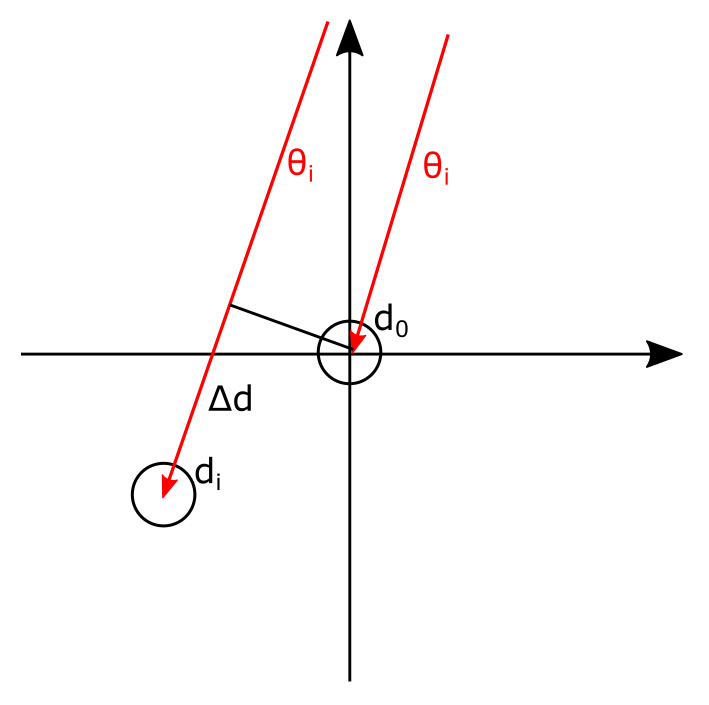
\includegraphics[width=\textwidth]{Images/direction.png}
    \caption{Opóźnienie fali na mikrofonie}
    \label{fig:direction}
\end{figure}

\newpage 

Poniższy model sygnału jest zaczerpnięty z \cite{Thiergart2013} i \cite{Braun2014}, z tą różnicą, że w tej pracy wszystkie zakłócenia traktowane są razem.

\noindent Zakłada się, że używanym czujnikiem jest macierz $M$ mikrofonów dookólnych rozłożonych na płaskiej powierzchnii w pozycjach $\{\bm{\mathrm{d}}_1...\bm{\mathrm{d}}_M\}$.

\noindent Na czujnik pada $L$ fal płaskich, gdzie $M > L$ ośrodku izotropowym i jednorodnym, w którym obecne są zakłócenia.Każda z fal nadbiega z kąta $\{{\theta}_1...{\theta}_L\}$ Model może być zapisany w dziedzinie STFT jako:
\begin{equation}
    \label{equation:2.1}
    \bm{\mathrm{x}}(k,n)
    =
    [\mathrm{X}(k,n,\bm{\mathrm{d}}_{1})
    ...
    \mathrm{X}(k,n,\bm{\mathrm{d}}_{M})]^{T}
\end{equation}
lub alternatywnie jako:
\begin{equation}
    \label{equation:2.2}
    \bm{\mathrm{x}}(k,n)=
    \sum_{l=1}^{L} \bm{\mathrm{x}}_{l}(k,n)
    + \bm{\mathrm{x}}_{\mathrm{n}}(k,n)
\end{equation}

\noindent gdzie $\bm{\mathrm{x}}_l(k,n)$ to wektor natężeń l-tej fali na poszczególnych mikrofonach a $\bm{\mathrm{x}}_{\mathrm{n}}(k,n)$ to wektor natężenia tła akustycznego na mikrofonach.
Oznacza to, że otrzymany na każdym z mikrofonów sygnał jest mieszaniną sygnału z kilku różnych źródeł i zakłóceń.

\begin{figure}[h]
    \centering
    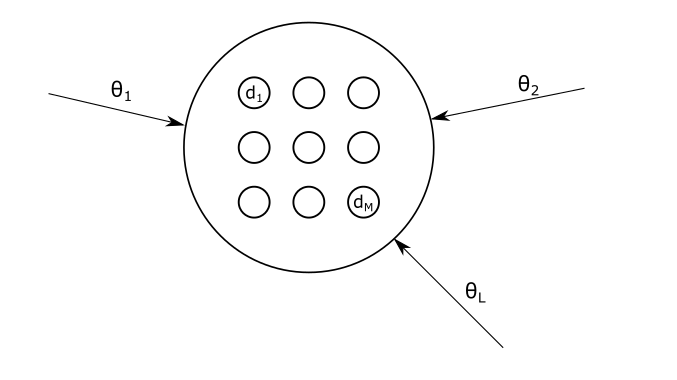
\includegraphics[width=\textwidth]{Images/model.png}
    \caption{Model systemu}
    \label{fig:model}
\end{figure}


\noindent Każdy z wektorów $\bm{\mathrm{x}}_l(k,n)$ może być opisany za pomocą równania:
\begin{equation}
    \label{equation:2.3}
    \bm{\mathrm{x}}_l(k,n)=
    \bm{\mathrm{a}}_l(k,n)X_{l}(k,n,\bm{\mathrm{d}}_{0})
\end{equation}
\noindent gdzie $\bm{\mathrm{a}}_l(k,n)X_{l}(k,n,\bm{\mathrm{d}}_{0})$ jest wartością natężenia l-tej fali w punkcie referencyjnym $\bm{\mathrm{d}}_0$. Często w publikacjach, na przykład w \cite{Braun2014} za punkt referencyjny jest wybierane położenie mikrofonu $\bm{\mathrm{d}}_1$. Autor pracy zdecydował się jednak na bardzej ogólne podejście do problemu.

\noindent W pracy zakłada się, że kierunek nadchodzenia fali nie jest znany ale znana jest ilość źródeł L w systemie.


\newpage
\section{Postawiony Problem}

W wyżej opisanym modelu mogą zostać zdefiniowane następujące potencjalne problemy:
\begin{itemize}
    \item Sygnał $\bm{\mathrm{x}}_{i}$ może charakteryzować się amplitudą różną od sygnału $\bm{\mathrm{x}}_{j}$ co będzie skutkować zagłuszaniem jednego z użytkowników systemu przez innego 
    \item Natężenie sygnału $\bm{\mathrm{x}}_{i}$ może mocno fluktować w czasie z uwagi na przykład na przybliżanie i oddalanie się mówcy od mikrofonów
    \item W systemie występuje tło akustyczne- niechciane zakłócenia, których wyeliminowanie jest pożądanym działaniem.
\end{itemize}

\noindent Autor pracy postawił sobie za cel minimalizację wyżej wymienionych problemów. Celem projektu jest uzyskanie takiego sygnału wyjściowego, w którym poziom głośności jest stały dla wszystkich mówców a występujące zakłócenia są jak najmniejsze.